\documentclass[11pt,a4paper]{article}
\usepackage[utf8]{inputenc}
\usepackage[T1]{fontenc}
\usepackage[spanish]{babel}
\usepackage{geometry}
\geometry{margin=2cm}
\usepackage{amsmath,amsfonts,amssymb}
\usepackage{booktabs}
\usepackage{graphicx}
\usepackage{xcolor}
\usepackage{fancyhdr}
\usepackage{titlesec}
\usepackage{float}

\definecolor{wasaffblue}{RGB}{0,82,147}

\pagestyle{fancy}
\fancyhf{}
\fancyhead[L]{\small\textcolor{wasaffblue}{WASAFF Consulting}}
\fancyhead[R]{\small\textcolor{wasaffblue}{Informe Ejecutivo}}
\fancyfoot[C]{\thepage}
\renewcommand{\headrulewidth}{0.4pt}

\titleformat{\section}{\normalfont\large\bfseries\color{wasaffblue}}{\thesection}{1em}{}

\begin{document}

% Portada
\begin{titlepage}
\centering
\vspace*{1.5cm}
{\Huge\bfseries\textcolor{wasaffblue}{Informe Ejecutivo}}\\[0.5cm]
{\LARGE Recuperación de Calor de Aceite de Compresores}\\[0.3cm]
{\Large CMPC Planta Santa Fe — Kaeser}\\[1.5cm]
\rule{0.8\textwidth}{0.5pt}\\[0.5cm]
{\large\textbf{WASAFF Consulting} — Mayo 2026}\\[1cm]
{\large Nivel de Servicio: Nivel 2 (Modelación Numérica Avanzada)}\\[1cm]
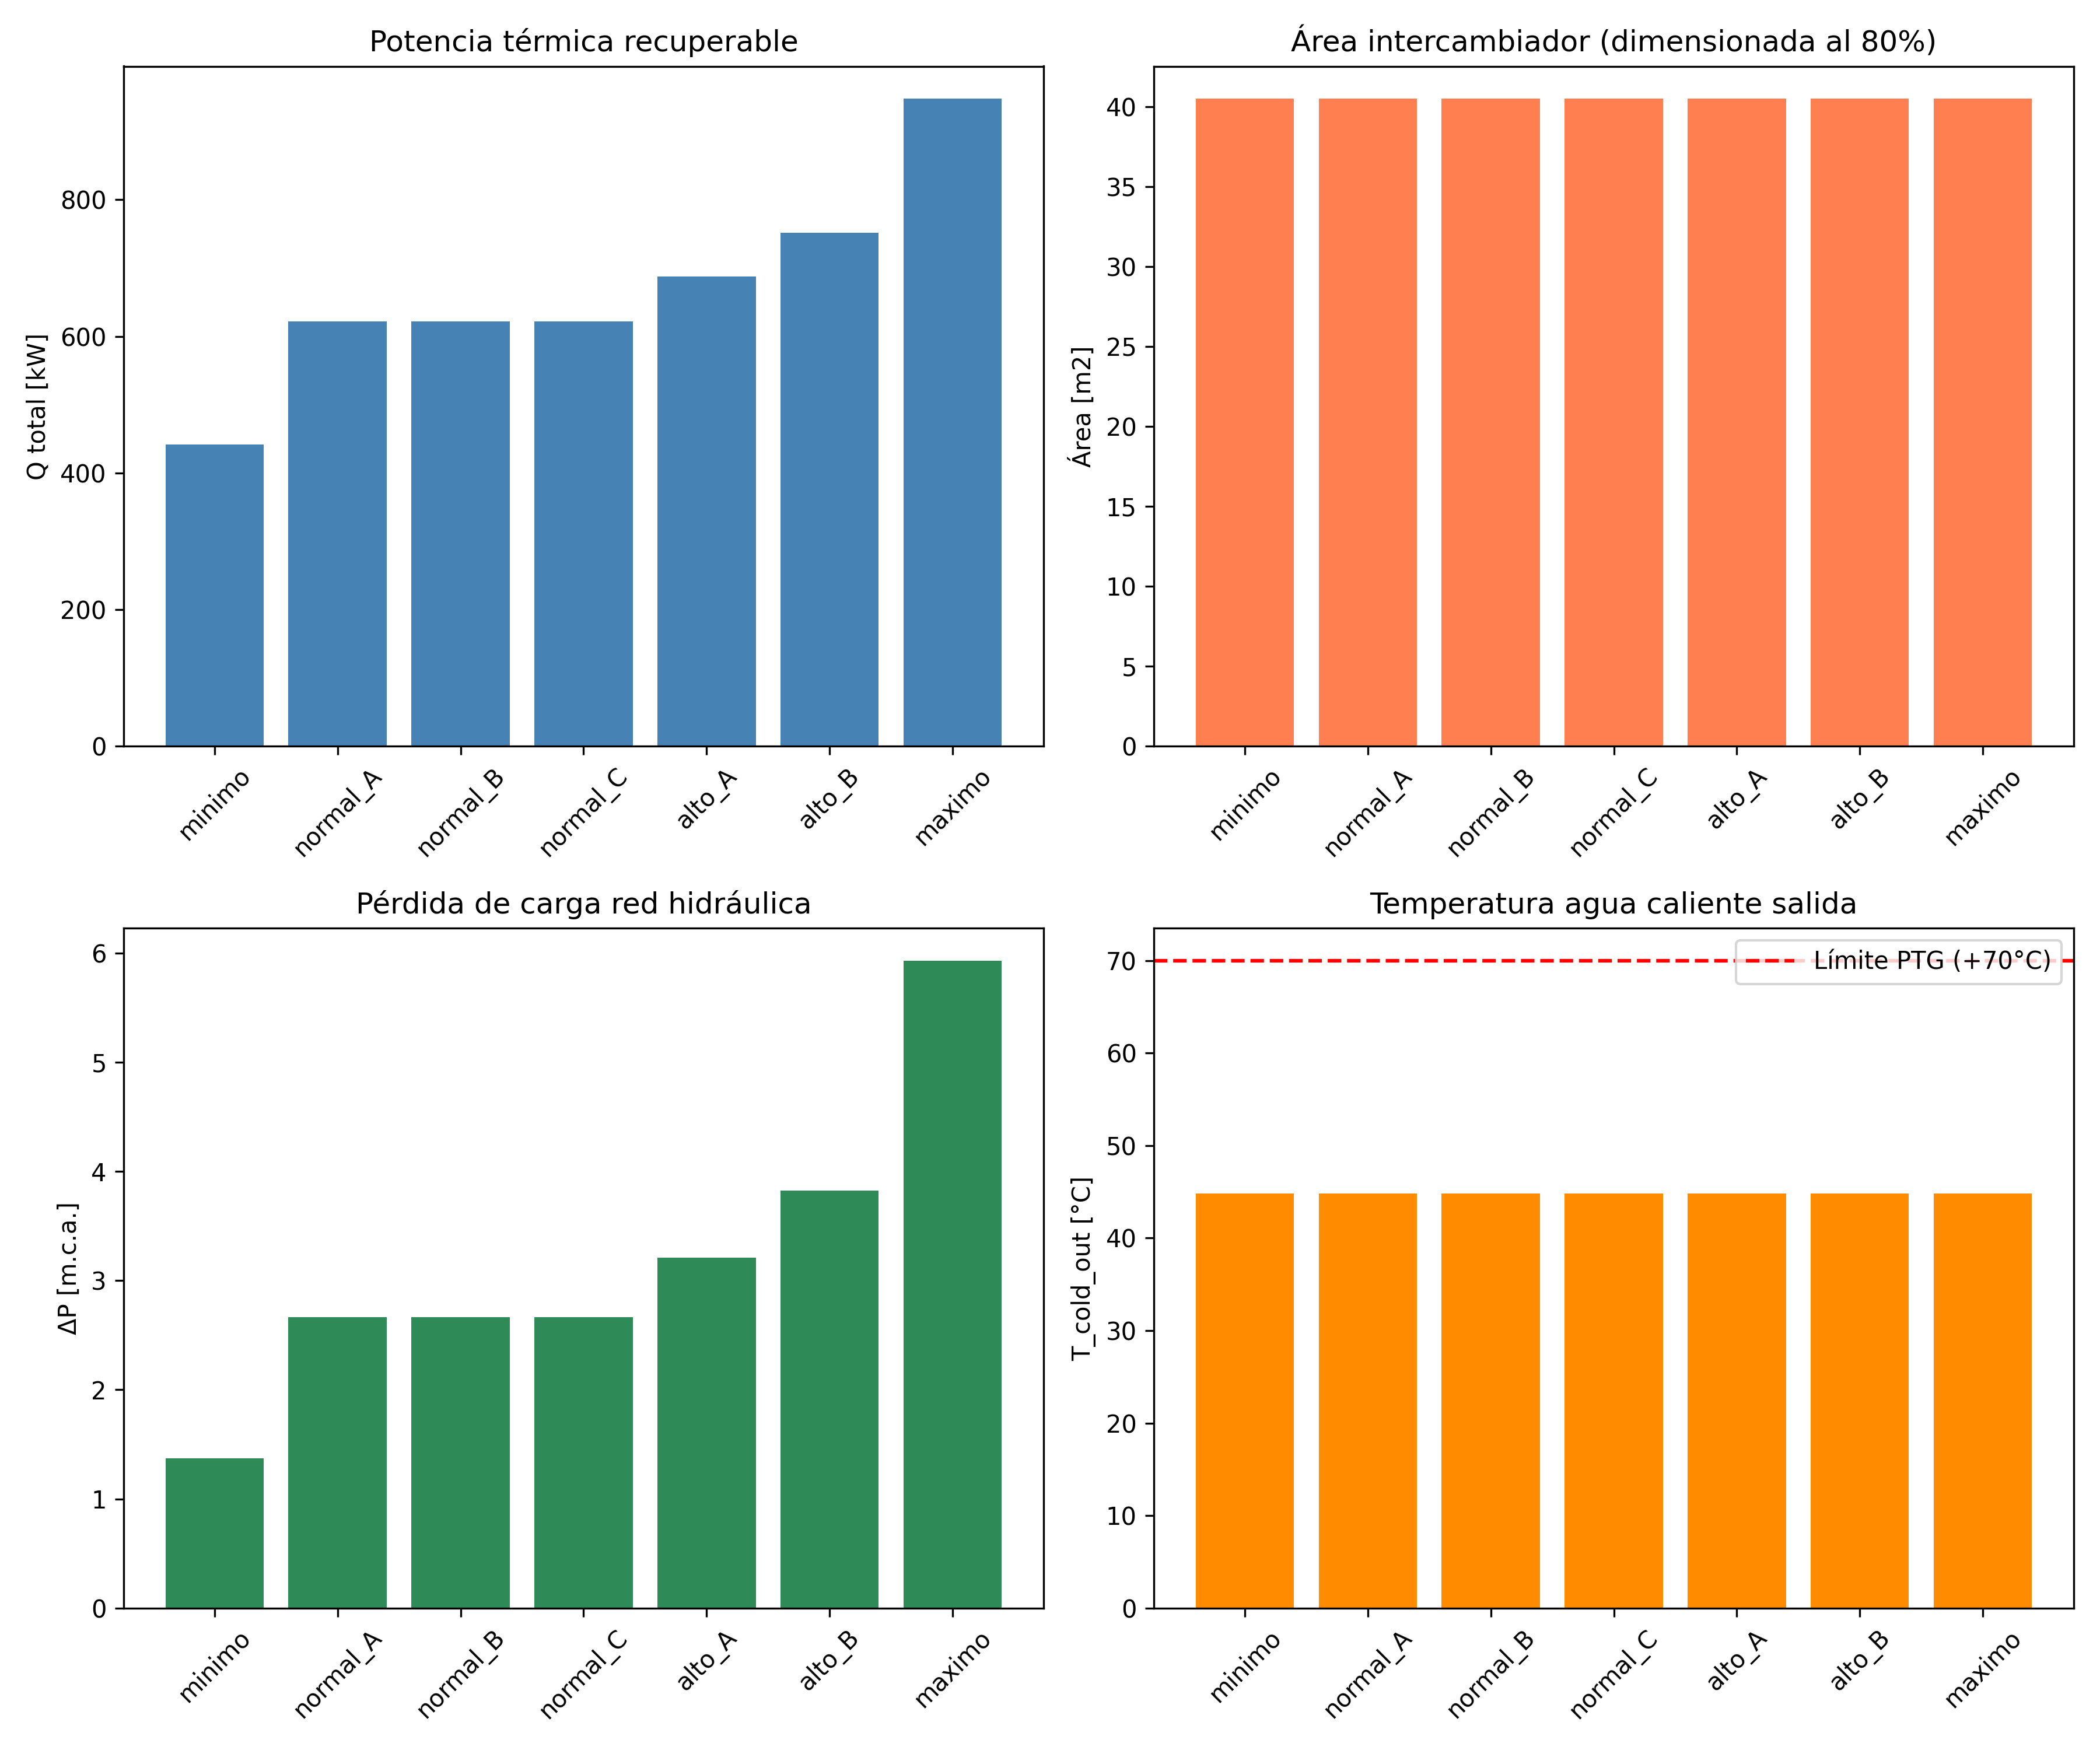
\includegraphics[width=0.7\textwidth]{../03_resultados/figuras/comparacion_escenarios.png}\\[0.5cm]
{\small Comparación de escenarios de operación}
\vfill
{\small Documento confidencial. Uso exclusivo del cliente.}
\end{titlepage}

\section*{Resumen}

Este informe ejecutivo resume los resultados del análisis de ingeniería de detalle para el sistema de recuperación de calor del aceite lubricante de compresores Kaeser en CMPC Santa Fe. El estudio utiliza modelación matemática avanzada (método $\varepsilon$-NTU, Darcy-Weisbach, RK45 transitorios, análisis de sensibilidad paramétrica) para dimensionar el sistema y cuantificar incertidumbres.

\section{Contexto del Proyecto}

La planta opera seis compresores de tornillo Kaeser con una potencia eléctrica instalada total de 1,885 kW. Aproximadamente el 80\% de esta energía se disipa como calor en el aceite lubricante (hasta $60^\circ\text{C}$). Este calor puede recuperarse para precalentar agua de proceso mediante un intercambiador de placas y una red hidráulica cerrada.

\section{Resultados Principales}

\begin{table}[H]
\centering
\caption{Resumen de resultados por escenario}
\begin{tabular}{@{}lcccc@{}}
\toprule
\textbf{Escenario} & \textbf{Pot. recuperada} & \textbf{Área IC} & \textbf{$\Delta P$} & \textbf{Bomba} \\
 & \textbf{[kW]} & \textbf{[m$^2$]} & \textbf{[m.c.a.]} & \textbf{[kW]} \\
\midrule
Mínimo (2 eq.) & 226 & 9.7 & 1.18 & 0.20 \\
Nominal (2 FSD) & 622 & 26.7 & 2.67 & 0.41 \\
Máximo (6 eq.) & 948 & 40.5 & 3.48 & 0.72 \\
\bottomrule
\end{tabular}
\end{table}

\textbf{Dinámica transitoria:} El tiempo de respuesta del sistema es de \textbf{2.4 minutos} (arranque en frío a estado nominal), lo cual es rápido y favorable para control.

\textbf{Incertidumbre:} El parámetro con mayor impacto en el dimensionamiento es el coeficiente global de transferencia $U$, seguido por la temperatura de aceite. Se recomienda un margen del 15\% sobre el área nominal.

\section{Recomendaciones}

\begin{enumerate}
  \item \textbf{Dimensionar intercambiador para 30--32 m$^2$} (15\% margen sobre nominal de 26.7 m$^2$).
  \item \textbf{Especificar placa SS316L} con $U_{\text{diseño}} \geq 3000\ \text{W/m}^2\text{K}$.
  \item \textbf{Bomba con VFD:} 5 m.c.a. de cabeza, control por variador de frecuencia.
  \item \textbf{Verificar in-situ:} Temperatura real del aceite ($T_{\text{hot}}$) antes de la compra.
  \item \textbf{Instrumentar:} Sensores de temperatura en ambos lados para calibración del modelo.
\end{enumerate}

\section{Inversión y ROI}

\begin{table}[H]
\centering
\begin{tabular}{@{}lr@{}}
\toprule
\textbf{Concepto} & \textbf{Valor} \\
\midrule
Inversión CAPEX estimada (Nivel 2) & USD \$350,000 -- \$540,000 \\
Ahorro energético anual (622 kW, 6,000 h/año) & USD \$280,000/año \\
Payback simple & 1.3 -- 1.9 años \\
Reducción emisiones CO$_2$ & $\sim$ 420 tCO$_2$/año \\
\bottomrule
\end{tabular}
\end{table}

\section{Próximos Pasos}

\begin{enumerate}
  \item Verificación de datos in-situ (temperaturas y caudales reales).
  \item Cálculo detallado de tuberías y soportes.
  \item Propuesta comercial formal con especificaciones técnicas.
  \item Opcional: validación FEniCS 2D y gemelo digital (Nivel 3).
\end{enumerate}

\vfill
\begin{center}
\rule{0.5\textwidth}{0.5pt}\\[0.3cm]
\textit{Felipe F. González P.}\\
Ingeniero Mecánico, MSc Candidate\\
WASAFF Consulting\\
\texttt{felipe@wasaff.cl}
\end{center}

\end{document}
